\chapter{Einleitung}
\label{cha:Einleitung}

\section{Motivation}
Für ERP-Softwarelösungen ist es wichtig möglichst auf die Wünsche des Kunden einzugehen. Dies beinhaltet auch die Anpassung an bereits existierende Konkurrenzlösungen. 
Um hier nicht für jeden Drittanbieter eine eigene Schnittstelle implementieren zu müssen, versucht man dies über eine Standardlösung, die international anerkannt ist, abzubilden. Hier hat sich speziell die XML (eXtensible Markup Language) etabliert. Die genannten Schnittstellen müssen stetig adaptiert und angepasst werden. 

Dies führt zu einem großen Entwicklungsaufwand, was die Validierung der einzelnen Felder bei der Kommunikation betrifft. 
Im Vordergrund steht hier die Basisüberprüfung wie die Datentypen der einzelnen Felder. Weiteres sollen Pflicht- und Informationsfelder validiert werden, aber auch einfache Geschäftsregeln sollen kontrolliert werden können. 
Zum Beispiel gibt es verschiedene Befehle, die als Attribut von einzelnen XML-Elementen gesetzt werden. Aufgrund dieser Ausprägung müssen verschiedene andere Elemente mitgeliefert werden. Fehlen solche Abhängigkeiten, ist die XML-Datei ungültig und soll nicht importiert werden.
Die so generierten Schemadateien sollen einerseits dem Fremdsystem zur Verfügung gestellt werden, als auch intern verwendet werden. 
Dem Fremdsystem soll es damit ermöglicht werden bereits von Inbetriebnahme der Schnittstelle beim Kunden, ihre Kommunikation mit BMD zu überprüfen. 

Hier bietet sich das XML Schema an, da dies ISO standardisiert ist und mit einer Vielzahl von Werkzeugen überprüft werden kann. 
Intern soll das XML Schema verwendet werden um Import-Dateien des Fremdsystem zu validieren und  um mögliche Fehlversuche zu verhindern. Deswegen wird das XML Schema auch intern generiert werden müssen, da die Schnittstelle jederzeit angepasst werden kann.
Da es oft eine Mehrzahl von Schnittstellen im Betrieb gibt, muss dies auch bei der Realisierung und Einbindung bedacht werden.


\section{Zielsetzung}
Das Ziel dieser Arbeit ist eine Beschreibung der notwendigen Schritte um aus Daten in einer relationalen Datenbank ein XML Schema zur Validierung von XML Dokumenten. Dabei sollen die Daten einer Beschreibung der einzelnen XML-Elementen entsprechen. Zum Beweis wird ein Prototyp erstellt, dessen Aus\-gabe eine XML-\-Schemadatei zur Validierung von XML-\-Dateien ist. Diese XML-Dateien dienen zum Austausch von Stamm-\- und Bewegungsdateien mit einem Fremd\-system. 
Die definierten Schnittstellen zu den Fremdsystemen variieren dabei sehr stark.
Als Basis der Überprüfung dient deswegen eine Auswahl von 
verschiedenen Feldern, wie in \ref{fig:Feldauswahl} dargestellt. 
Diese Felder repräsentieren jeweils eine Spalte einer relationalen Datenbank. 
Jede Auswahl ist wiederum in einer Tabelle gespeichert. 
Es müssen sowohl Oracle und Microsoft SQL Server unterstützt werden, da auch das ERP-System beide Datenbank-Systeme unterstützt. 
Konkret soll diese Software in das Modul der PPS (Produktionsplanungs- und Steuerungssystem) vom BMD Systemhaus GesmbH integriert werden. 
Dies bedeutet, dass das neue System keine eigen\-ständige Software sein soll oder muss. 
Den Fremdsystemen werden nur die Schemadateien zur Verfügung gestellt.

\begin{figure}
    \centering
    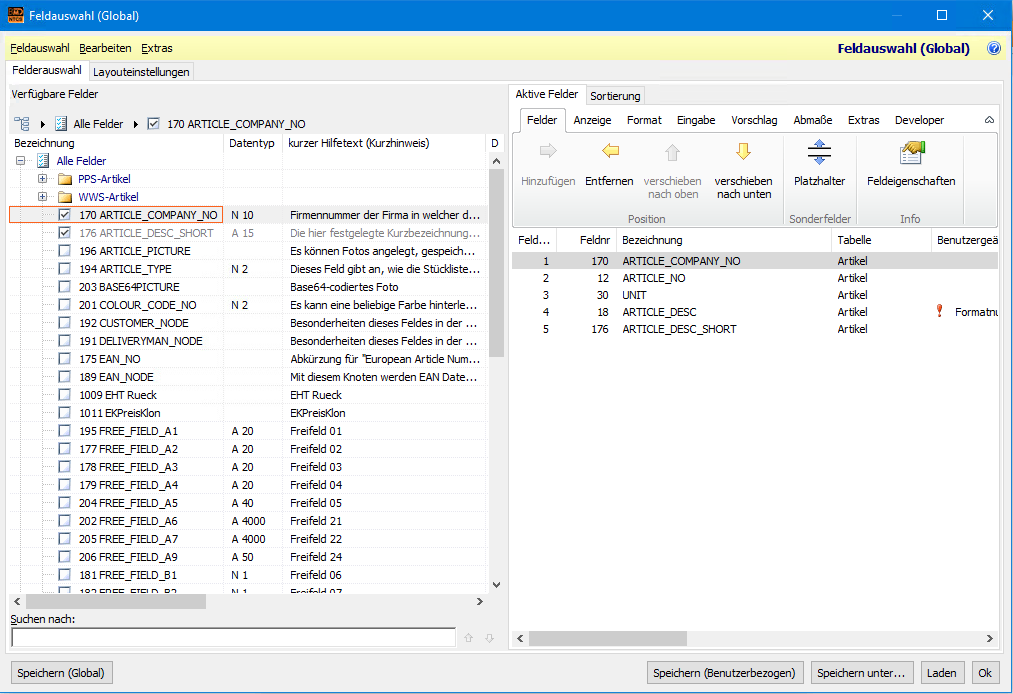
\includegraphics[width=.95\textwidth]{images/Feldauswahl.png}
    \caption{Definition Schnittstelle in BMD}
    \label{fig:Feldauswahl}
\end{figure}
